\documentclass[conference]{IEEEtran}
\usepackage{cite}
\usepackage{amsmath,amssymb,amsfonts}
\usepackage{algorithmic}
\usepackage{graphicx}
\usepackage{textcomp}
\usepackage{xcolor}
\def\BibTeX{{\rm B\kern-.05em{\sc i\kern-.025em b}\kern-.08em
    T\kern-.1667em\lower.7ex\hbox{E}\kern-.125emX}}
\begin{document}
\selectlanguage{english}

\title{Discovering Digital Art Collections using Link-Traversal–based Query Processing}

\author{\IEEEauthorblockN{Martijn Bogaert}
\IEEEauthorblockA{
\textit{Ghent University}\\
Ghent, Belgium \\
martijn.bogaert@ugent.be}}

\maketitle

\begin{abstract}
This master's thesis explores the exploration of digital art collections through Link-Traversal-based Querying, with a focus on the \textit{Collections of Ghent}. The Comunica platform plays a key role in harnessing valuable data in RDF format, although some links pose challenges with RDF compatibility. Two web application ideas are proposed to assist both non-technical users and professionals in exploring the CoGhent collection. The ultimate goal is to associate discovered data with IIIF Manifests for visualization, thus increasing the accessibility of art collections.
\end{abstract}

\begin{IEEEkeywords}
Linked Data, Link Traversal, LTQP, CoGhent, IIIF
\end{IEEEkeywords}

\section*{Introduction}
TODO

\section{Related Work}
TODO

\subsection{Collections of Ghent}
TODO

\subsection{International Image Interoperability Framework}
TODO

\subsection{Link-Traversal-based Query Processing}
TODO

\section{CoGhent Data and Link Traversal}
TODO

\subsection{CoGent Data Sources}
TODO

\subsection{Comunica Link Traversal Engine Configuration}
TODO

\subsection{Links to Follow}
TODO

\section{Tools for Query Building}
TODO

\subsection{Building Queries from Predicate Sequences}
TODO

\subsection{User-centric Tools}
TODO

\section{Handling Query Results}
TODO

\subsection{Visualizing Query Results}
TODO

\subsection{Saving Query Results}
TODO

\section*{Acknowledgment}
TODO

% \bibliographystyle{IEEEtran}
% \bibliography{references}

\end{document}


% \begin{table}[htbp]
% \caption{Table Type Styles}
% \begin{center}
% \begin{tabular}{|c|c|c|c|}
% \hline
% \textbf{Table}&\multicolumn{3}{|c|}{\textbf{Table Column Head}} \\
% \cline{2-4} 
% \textbf{Head} & \textbf{\textit{Table column subhead}}& \textbf{\textit{Subhead}}& \textbf{\textit{Subhead}} \\
% \hline
% copy& More table copy$^{\mathrm{a}}$& &  \\
% \hline
% \multicolumn{4}{l}{$^{\mathrm{a}}$Sample of a Table footnote.}
% \end{tabular}
% \label{tab1}
% \end{center}
% \end{table}

% \begin{figure}[htbp]
% \centerline{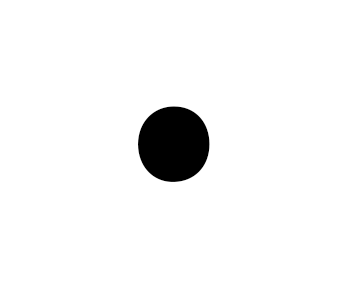
\includegraphics{fig1.png}}
% \caption{Example of a figure caption.}
% \label{fig}
% \end{figure}